% =================================================================================================
% File:			client_tier/model/data.tex
% Description:	Defiinisce la sezione relativa al front-end dell'applicazione
% Created:		2015-04-10
% Author:		Tesser Paolo
% Email:		tesser.paolo@mashup-unipd.it
% =================================================================================================
% Modification History:
% Version		Modifier Date		Change											Author
% 0.0.1 		2015-04-10 			creato scheletro								Tesser Paolo
% =================================================================================================
% 0.0.2			2015-04-11			scheletro classi contenuti nei package			Tesser Paolo
% =================================================================================================
%

% CONTENUTO DEL CAPITOLO
%

\subsubsection{bdsm\_app::client::model::data} % (fold)
\label{ssub:bdsm_app_client_model_data}
\begin{figure}[htbp]
	\centering
	\centerline{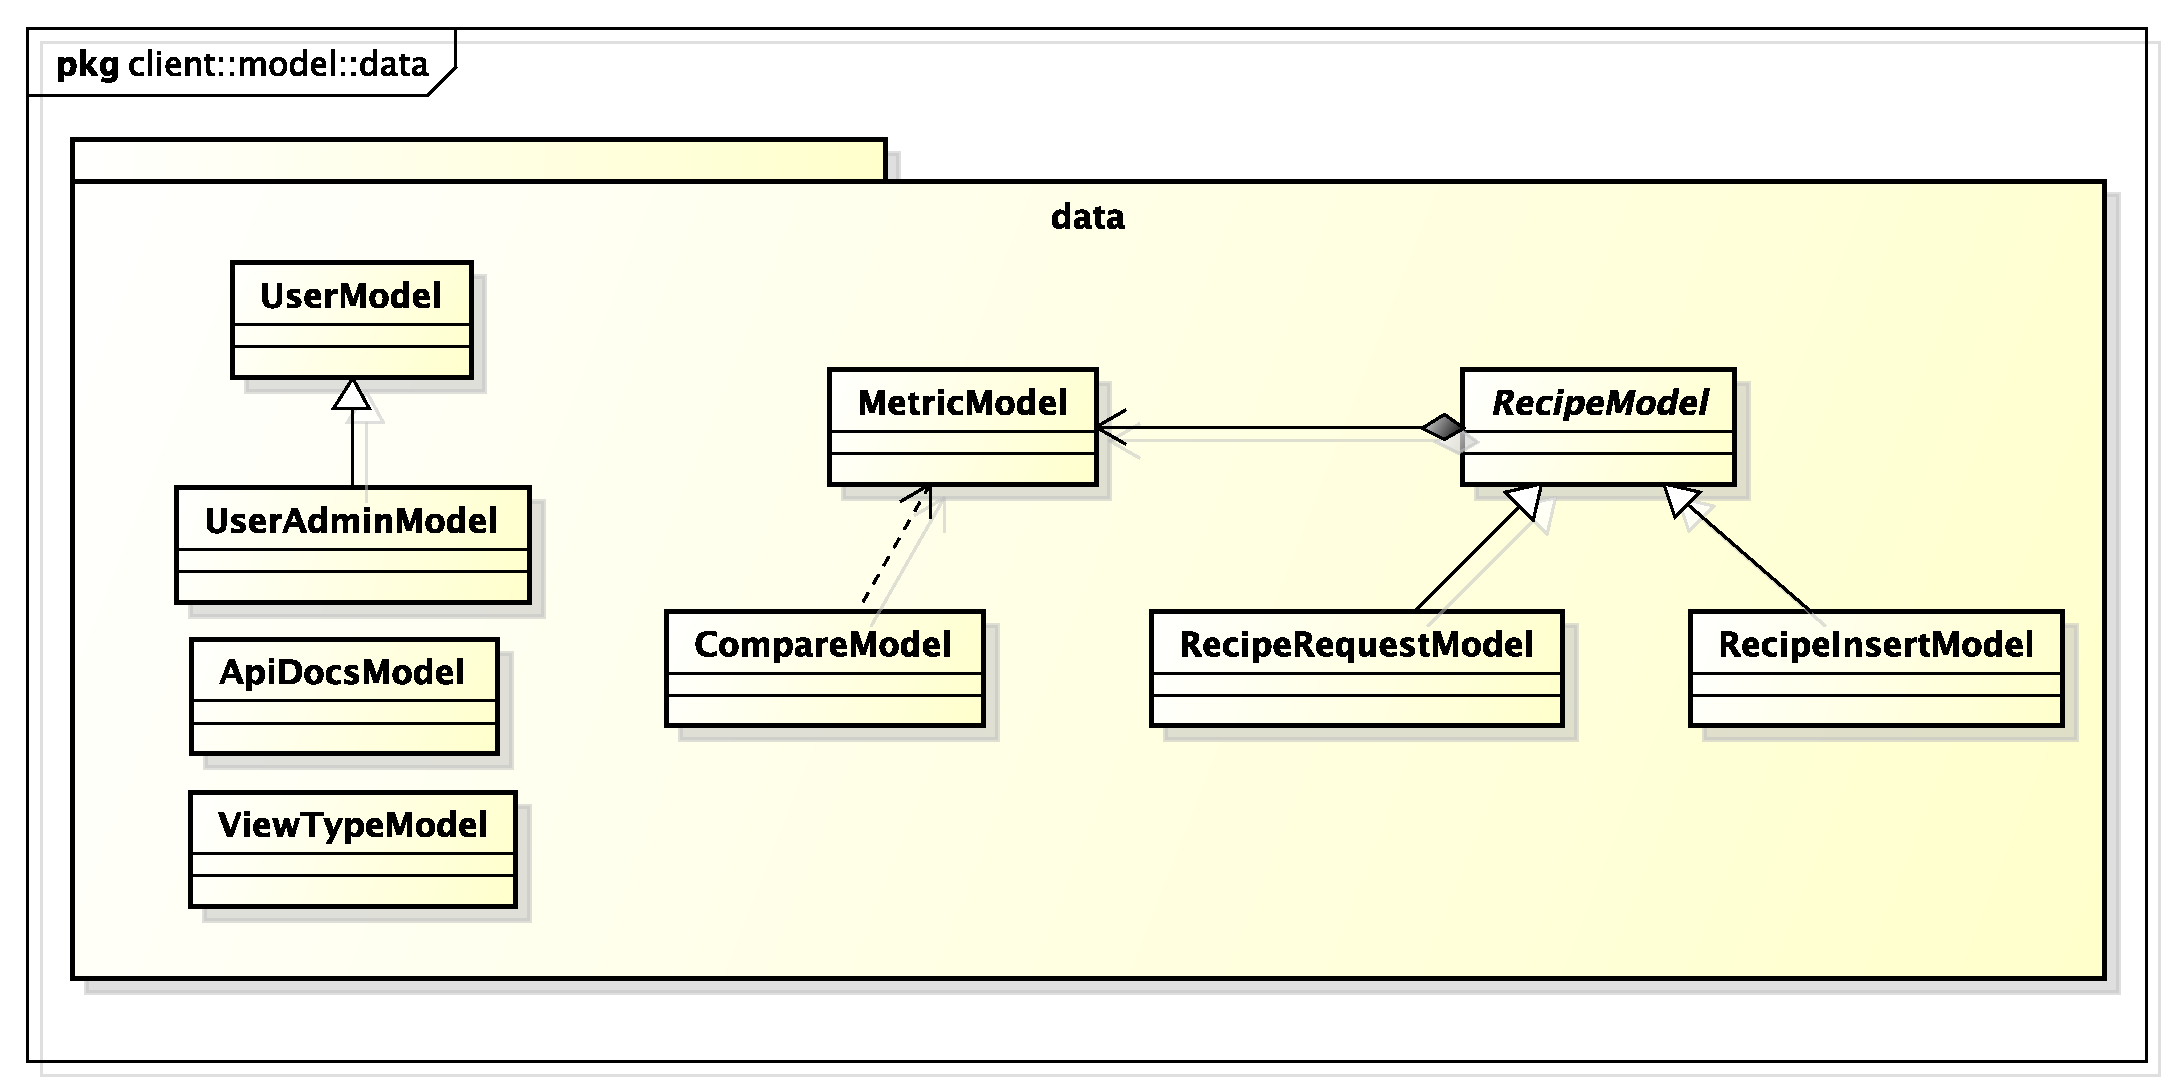
\includegraphics[scale=0.5]{./images/client_model_data.pdf}}
	\caption{Package - client::model::data}
\end{figure}

\begin{itemize}
	\item \textbf{Descrizione}: è il package c;
	\item \textbf{Padre}: client::model
	\item \textbf{Interazione con altri componenti}:
		\begin{itemize}
			\item client::model::services
			\item client::controller
		\end{itemize}

	\paragraph{Classi} % (fold)

		\subparagraph{client::model::data::ViewTypeModel} % (fold)
		\label{subp:client_model_data_viewtypemodel}
			\begin{itemize}
				\item \textbf{Descrizione}: [TO DO];
				\item \textbf{Utilizzo}: [TO DO];
				\item \textbf{Classi ereditate}: [TO DO];
				\item \textbf{Relazioni con altre classi}: [TO DO].
			\end{itemize}
		% subparagraph client_model_data_viewtypedata (end)

		\subparagraph{client::model::data::ApiDocsModel} % (fold)
		\label{subp:client_model_data_apidocsmodel}
			\begin{itemize}
				\item \textbf{Descrizione}: [TO DO];
				\item \textbf{Utilizzo}: [TO DO];
				\item \textbf{Classi ereditate}: [TO DO];
				\item \textbf{Relazioni con altre classi}: [TO DO].
			\end{itemize}
		% subparagraph client_model_data_apidocsmodel (end)


		\subparagraph{client::model::data::UserModel} % (fold)
		\label{subp:client_model_data_user}
			\begin{itemize}
				\item \textbf{Descrizione}: [TO DO];
				\item \textbf{Utilizzo}: [TO DO];
				\item \textbf{Classi ereditate}: [TO DO];
				\item \textbf{Relazioni con altre classi}: [TO DO].
			\end{itemize}
		% subparagraph client_model_data_user (end)

		\subparagraph{client::model::data::UserAdminModel} % (fold)
		\label{subp:client_model_data_useradminmodel}
			\begin{itemize}
				\item \textbf{Descrizione}: [TO DO];
				\item \textbf{Utilizzo}: [TO DO];
				\item \textbf{Classi ereditate}: [TO DO];
				\item \textbf{Relazioni con altre classi}: [TO DO].
			\end{itemize}
		% subparagraph client_model_data_useradminmodel (end)

		\subparagraph{client::model::data::RecipeModel} % (fold)
		\label{subp:client_model_data_recipe}
			\begin{itemize}
				\item \textbf{Descrizione}: [TO DO];
				\item \textbf{Utilizzo}: [TO DO];
				\item \textbf{Classi ereditate}: [TO DO];
				\item \textbf{Relazioni con altre classi}: [TO DO].
			\end{itemize}
		% subparagraph client_model_data_recipe (end)

		\subparagraph{client::model::data::RecipeRequestModel} % (fold)
		\label{subp:client_model_data_reciperequestmodel}
			\begin{itemize}
				\item \textbf{Descrizione}: [TO DO];
				\item \textbf{Utilizzo}: [TO DO];
				\item \textbf{Classi ereditate}: [TO DO];
				\item \textbf{Relazioni con altre classi}: [TO DO].
			\end{itemize}
		% subparagraph client_model_data_reciperequestmodel (end)

		\subparagraph{client::model::data::RecipeInsertModel} % (fold)
		\label{subp:client_model_data_recipeinsertmodel}
			\begin{itemize}
				\item \textbf{Descrizione}: [TO DO];
				\item \textbf{Utilizzo}: [TO DO];
				\item \textbf{Classi ereditate}: [TO DO];
				\item \textbf{Relazioni con altre classi}: [TO DO].
			\end{itemize}
		% subparagraph client_model_data_recipeinsertmodel (end)

		\subparagraph{client::model::data::MetricModel} % (fold)
		\label{subp:client_model_data_metricmodel}
			\begin{itemize}
				\item \textbf{Descrizione}: [TO DO];
				\item \textbf{Utilizzo}: [TO DO];
				\item \textbf{Classi ereditate}: [TO DO];
				\item \textbf{Relazioni con altre classi}: [TO DO].
			\end{itemize}
		% subparagraph client_model_data_metricmodel (end)

		\subparagraph{client::model::data::CompareModel} % (fold)
		\label{subp:client_model_data_comparemodel}
		
		% subparagraph client_model_data_comparemodel (end)


\end{itemize}
% subsubsection bdsm_app_client_model_data (end)